\subsection{Iterations}

The following four prototype iterations shown on figure \ref{fig:v1} to \ref{fig:v5}, depict an exploded view of the design on the left, and the physical version on the right. There is one major change in design during the process from prototype two to three, but they have all one thing in common: the journal is meant to be fixed on top of an acrylic sheet. \\
The first two prototype ideas shown on figures \ref{fig:v1} and \ref{fig:v2} were made entirely with acrylic sheets cut with a laser-cutter, and the two remaining ones, a mix of laser cutting, and 3D printing.

\subsubsection{First iteration}
The first prototype on figure \ref{fig:v1} was designed to accommodate eight banks of 4 x 1,5V AAA batteries. Compartments for each electronic component were made to place them on a flat surface, and reduce thickness. A box on the left of the journal was meant to hold LEDs. 

\begin{figure}[h]
\setlength{\belowcaptionskip}{-5mm}
\begin{minipage}[b]{.5\textwidth}
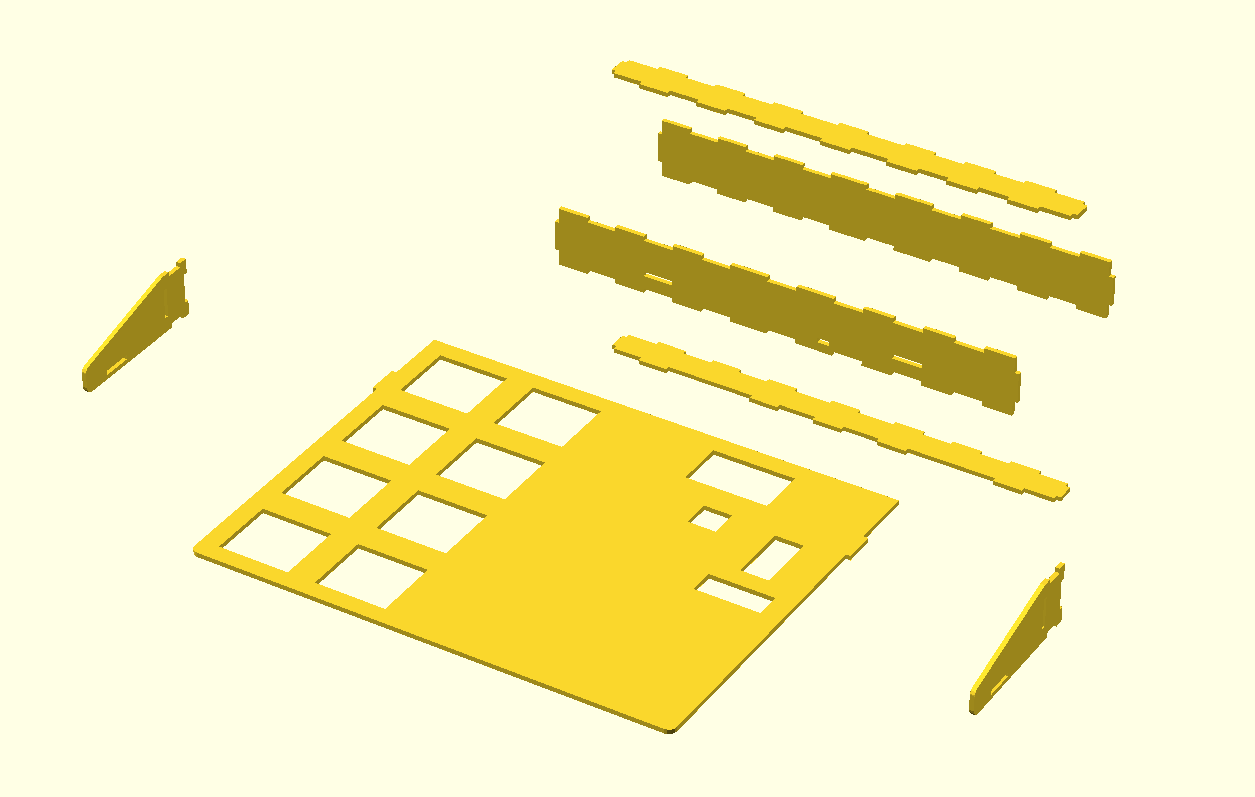
\includegraphics[width=1.05\textwidth]{figures/iterations/v1.png}
\end{minipage}
\begin{minipage}[b]{.5\textwidth}
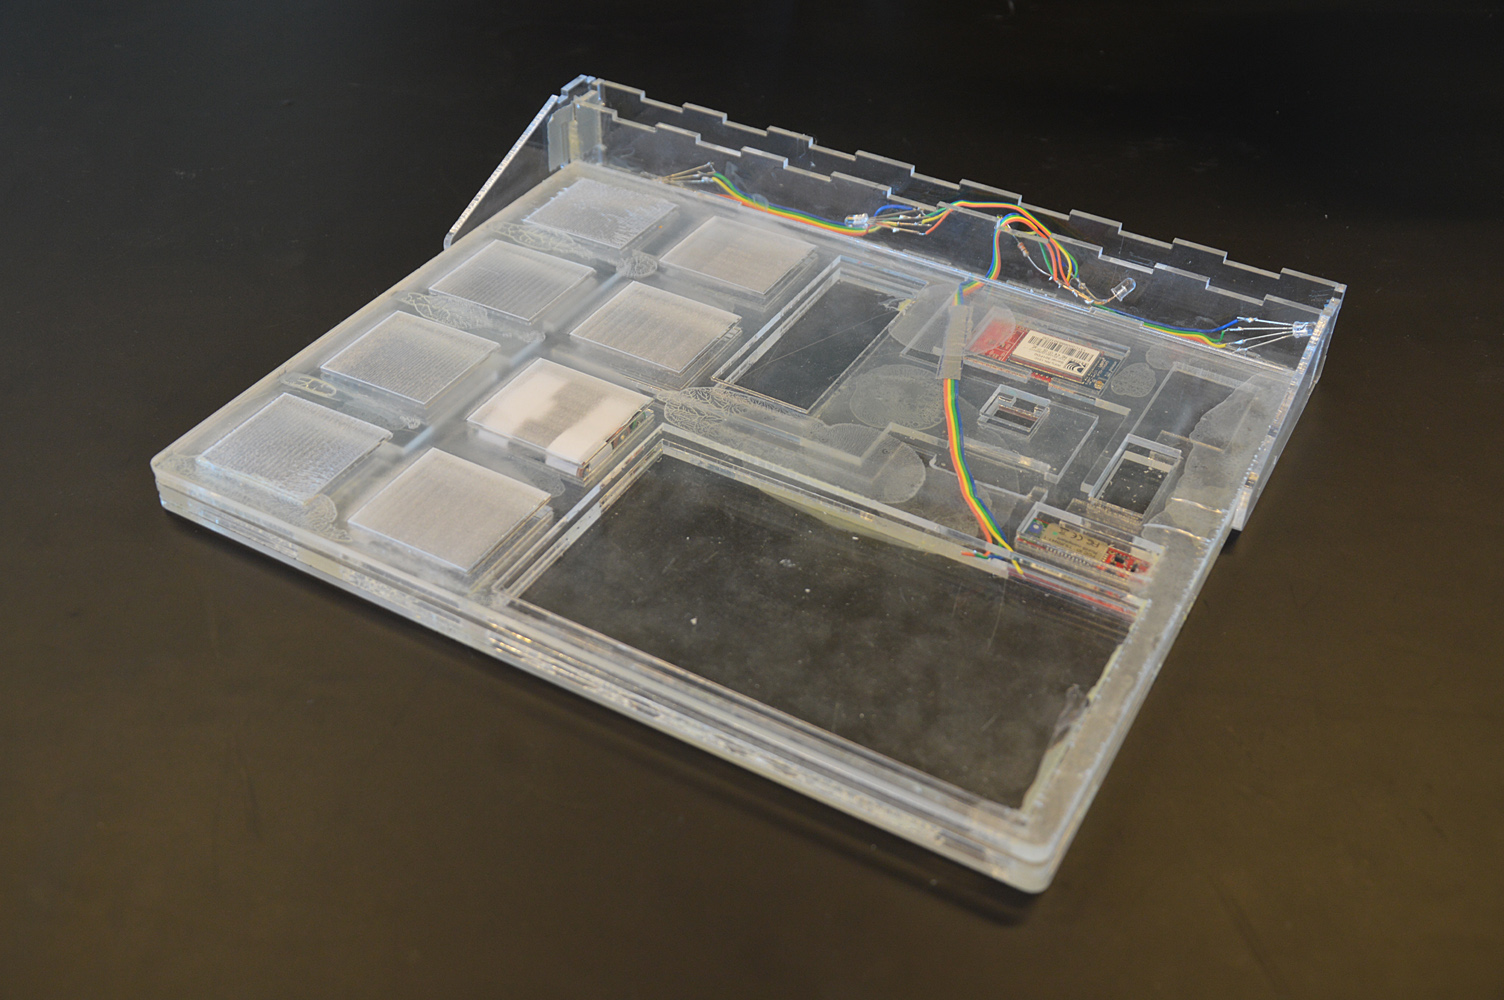
\includegraphics[width=1\textwidth]{figures/iterations/v1-photo.jpg}
\end{minipage}
\caption{\small {\it {The first prototype idea}}} 
\label{fig:v1}
\end{figure}

This design had many flaws however -- the list below describes the various issues.

\begin{itemize} \itemsep0em
  \item It felt heavy, and the weight exceeded 500g.
  \item The sharp edges from the laser-cut acrylic were slightly uncomfortable.
  \item The sheets were glued together, and made the case impossible to open.
  \item The glueing process is tedious because of the tools needed, and the hardening takes 24h.
  % \item Compartments were engraved with the laser-cutter, which requires constant supervision of the cutting.
  \item Problems with displacement of compartments from the different acrylic sheets.
  \item No charging possibility.
  \item Wiring of components was difficult.
  \item The side piece made it difficult to open the journal.
\end{itemize}

A few positive characteristics were observed:
\begin{itemize} \itemsep0em
  \item Removal of protruding bolts.
  \item Reduced thickness by 15mm.
\end{itemize}

% -------------------

\subsubsection{Second iteration}
The second prototype took the previous downsides into consideration, and produced the device shown on figure \ref{fig:v2}. The idea here, is that the electronics were to be moved to a box at the bottom of the journal, in order to make the journal feel less bulky while holding it.

\begin{figure}[h]
\setlength{\belowcaptionskip}{0mm}
\begin{minipage}[b]{.5\textwidth}
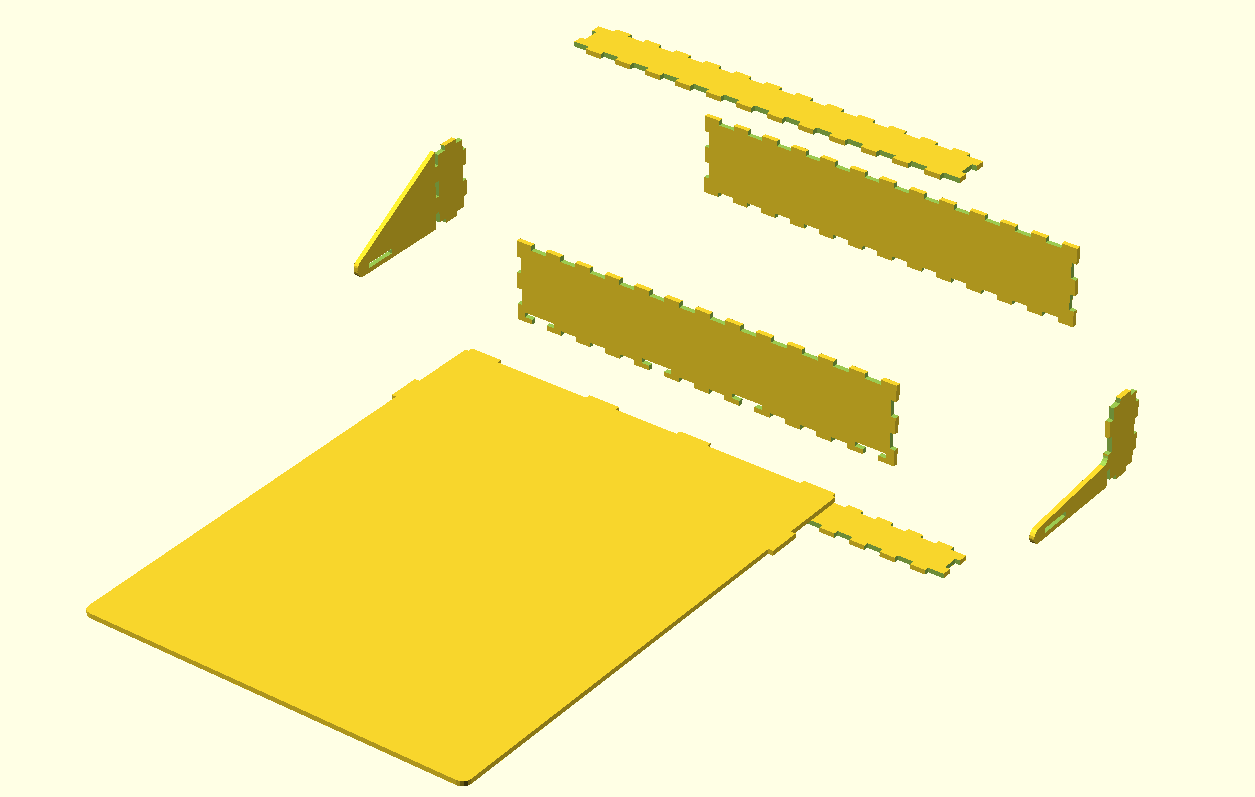
\includegraphics[width=1.05\textwidth]{figures/iterations/v3.png}
\end{minipage}
\begin{minipage}[b]{.5\textwidth}
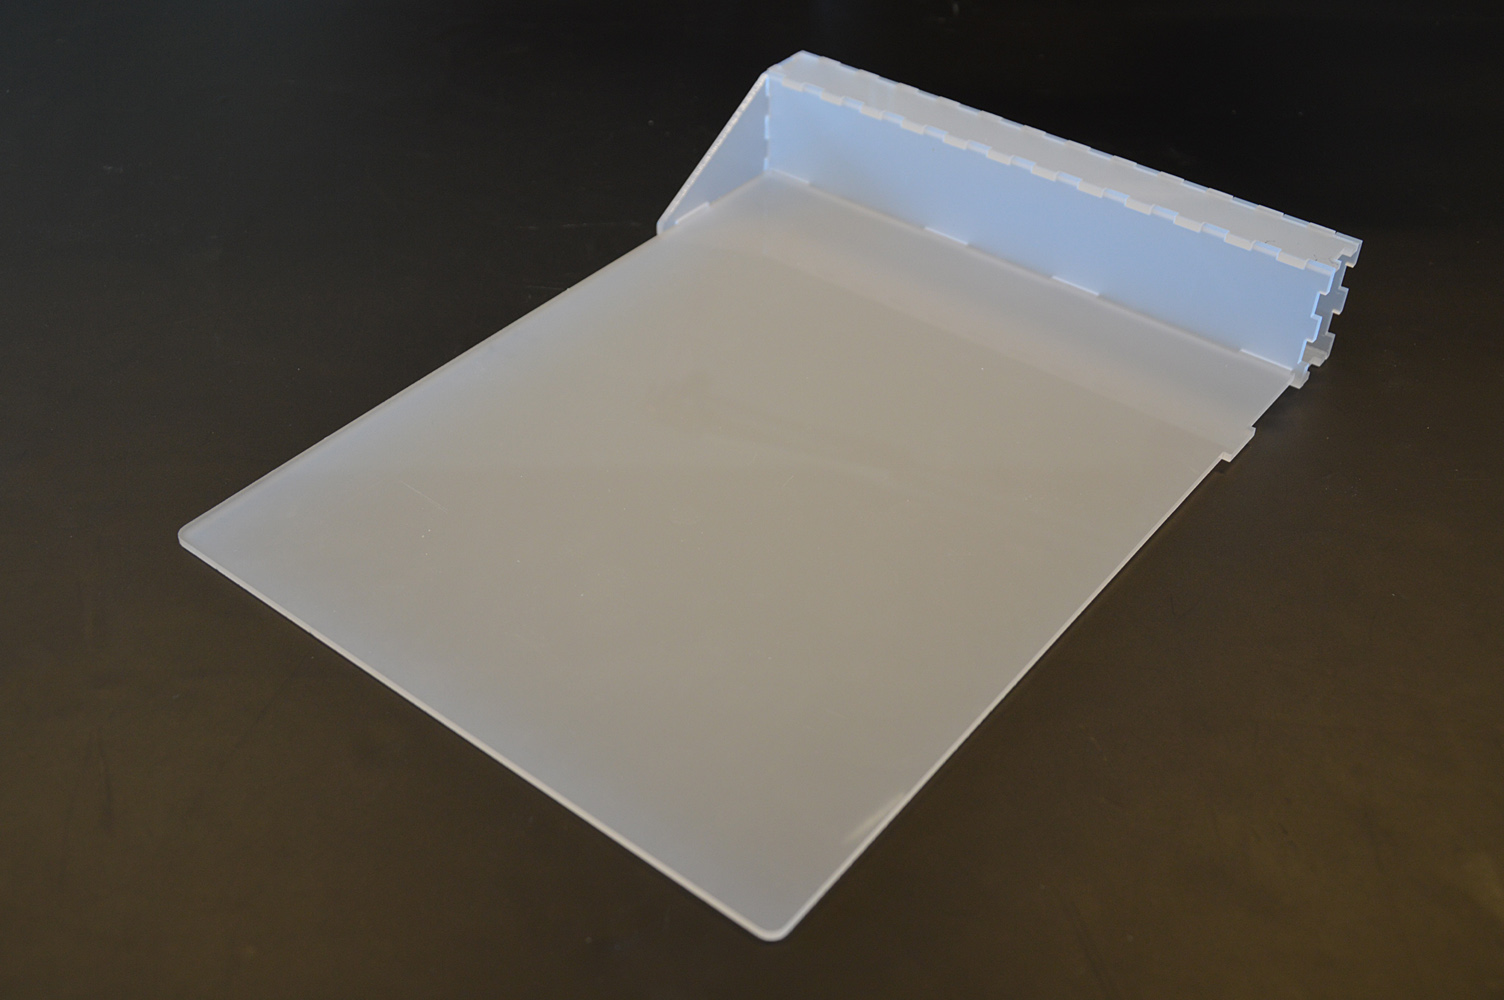
\includegraphics[width=1\textwidth]{figures/iterations/v3-photo.jpg}
\end{minipage}
\caption{\small {\it {The second prototype idea}}} 
\label{fig:v2}
\end{figure}

Following are the issues found with this design:

\begin{itemize} \itemsep0em
	\item Not very pleasant to hold, as the box holding the electronics ended up getting in the way of the user.
	\item Impossibility of performing maintenance, due to the acrylic being glued.
	\item Structurally unsound design - attachment of box to the sheet was flimsy, and broke easily.
	\item No charging possibility.
	\item The weight distribution would have been very uneven, due to the placement of box at the bottom.
\end{itemize}

This prototype was discarded before an attempt to place the electronics in the box, due to the obvious disadvantages. The technique of laser-cutting acrylic sheets and using glue to attach them together proved to be a slow and tedious task. Due to the difficulty of using screws to assemble the parts and using glue instead, made the designs unmaintainable. Complex laser-cut acrylic parts also tended to become brittle, so a rethinking of the design was in order. Using acrylic wasn't out of the question, but the complexity of those parts had to be reduced, and the use of 3D printed PLA for those parts were later introduced. \\

% -------------------

\subsubsection{Third iteration}

Figure \ref{fig:v3} depicts the third prototype. The electronics were moved to a new 3D printed container made of PLA. The latter was further divided into smaller compartments made for housing the various electronic components. The container had a lid that was screwed on top.

\begin{figure}[h]
\setlength{\belowcaptionskip}{0mm}
\begin{minipage}[b]{.5\textwidth}
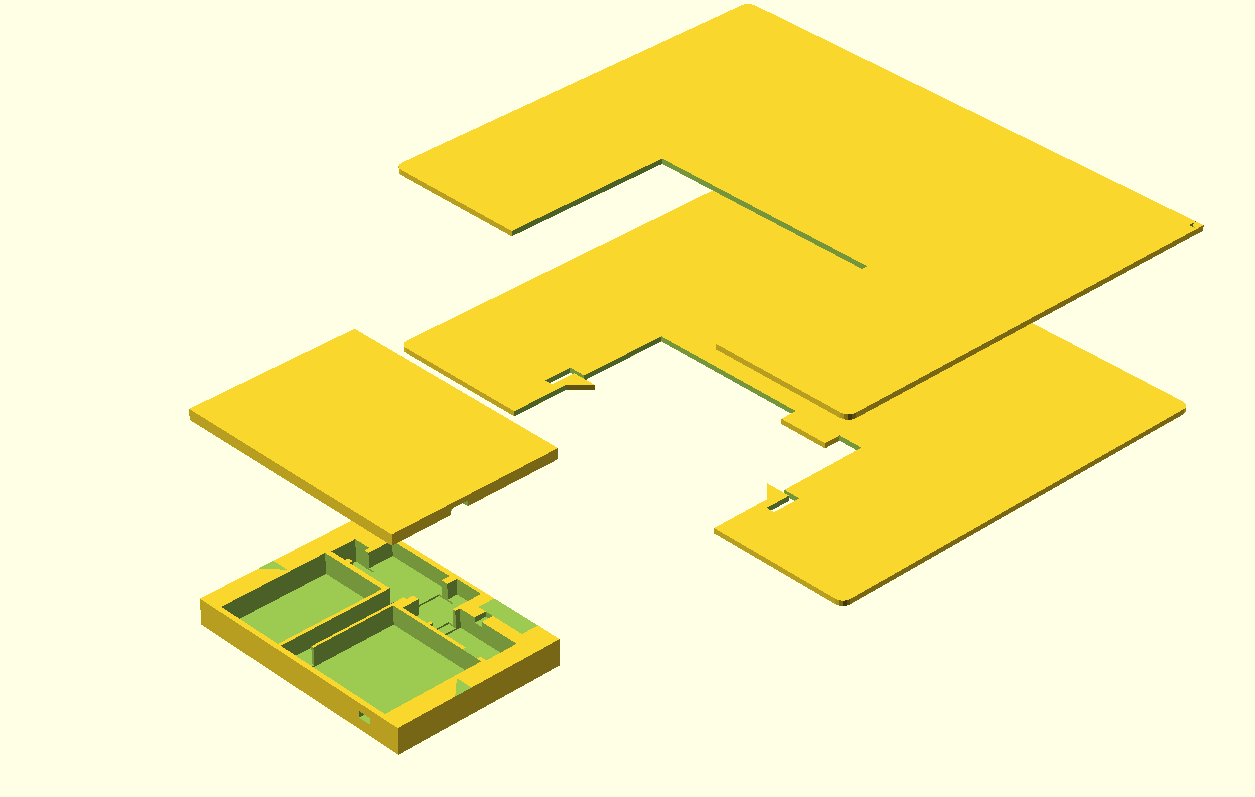
\includegraphics[width=1.05\textwidth]{figures/iterations/v4.png}
\end{minipage}
\begin{minipage}[b]{.5\textwidth}
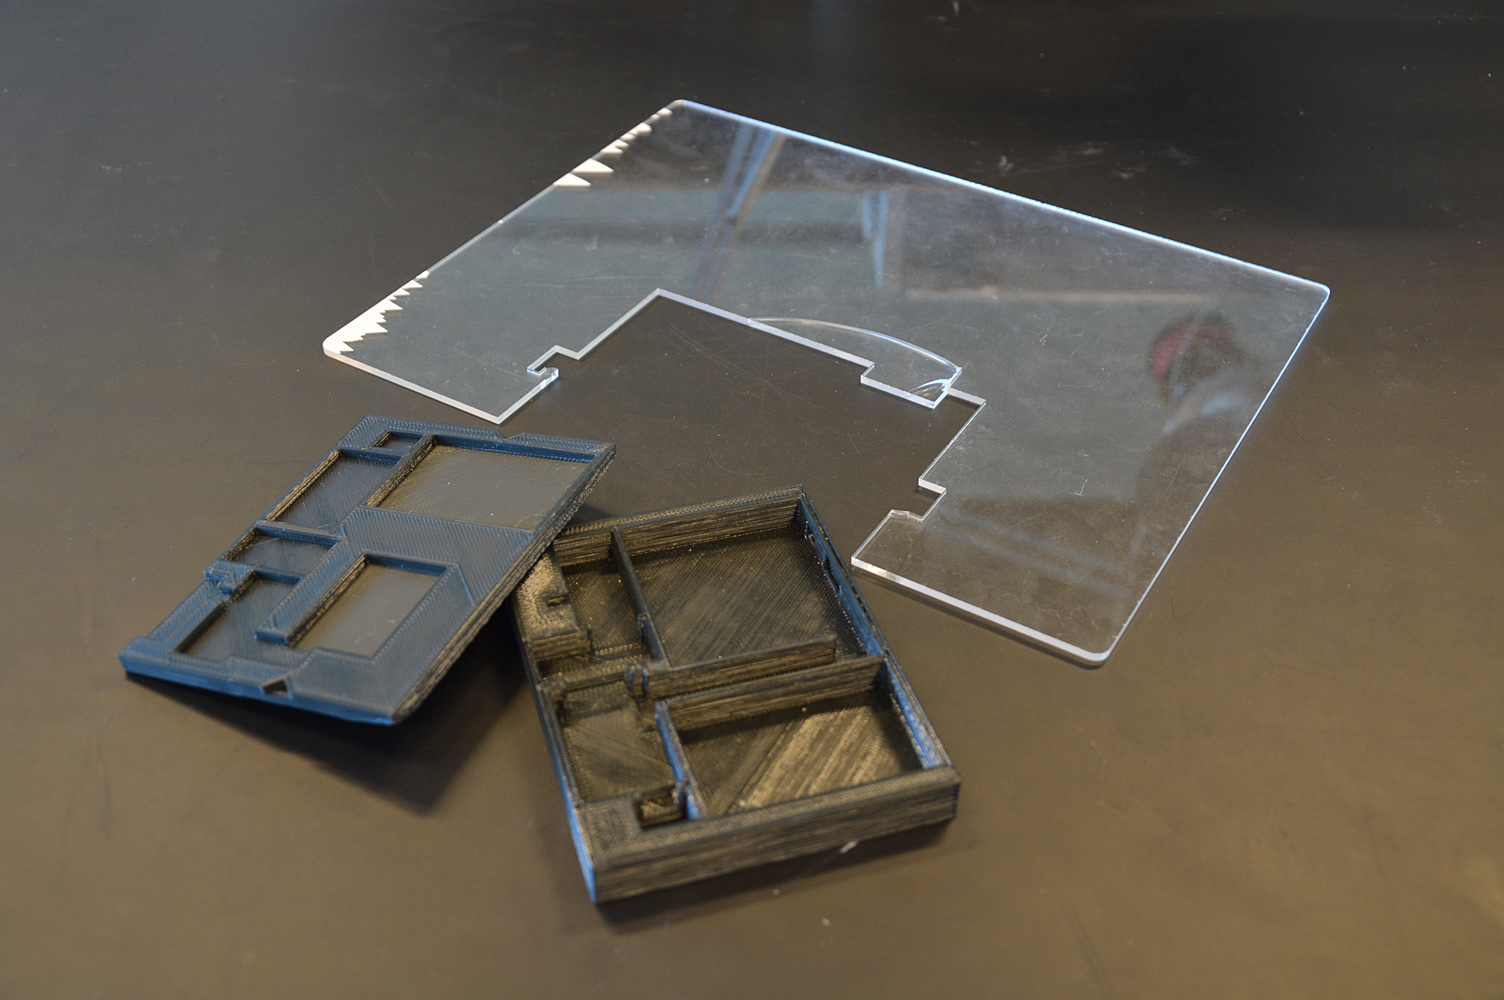
\includegraphics[width=1\textwidth]{figures/iterations/v4-photo.jpg}
\end{minipage}
\caption{\small {\it {The third prototype idea}}} 
\label{fig:v3}
\end{figure}

The box was also designed to be slid into a sheet of acrylic. Two small protruding triangles where cut in the acrylic sheets in order for them to bend, and the box would then ``click'' into place. The purpose of such system is to make maintainability easier - one would simply have to slide the box out, perform a software update and slide it back in. This was however difficult to get right, and the bending acrylic ended up breaking quickly. Figure \ref{fig:v3} shows the broken acrylic on the right. Two holes on the side were also added to hold an RGB LED, and the other to hold the USB charger intake.

Following are the issues found with this design:

\begin{itemize} \itemsep0em
  \item The compartments for the electronic components ended up making the wiring of the latter unnecessary complex.
  \item The click system was difficult to achieve with acrylic.
  \item The chosen RGB LED's colours were difficult to discern.
\end{itemize}

This prototype attempted however to resolve many problems found in the previous iterations, and the following positive attributes were observed:

\begin{itemize} \itemsep0em
  \item Comfortable to hold.
  \item Maintenance is easier to perform.
  \item Battery charging via standard mini-USB cable.
  \item The electronics were moved out of the way of the user.
  \item Better weight distribution when holding the journal.
  \item 3D printing opened up possibilities to radically change the design.
\end{itemize}

% -------------------

% \begin{figure}[h]
% \begin{minipage}[b]{7.5cm}
% \centering
% 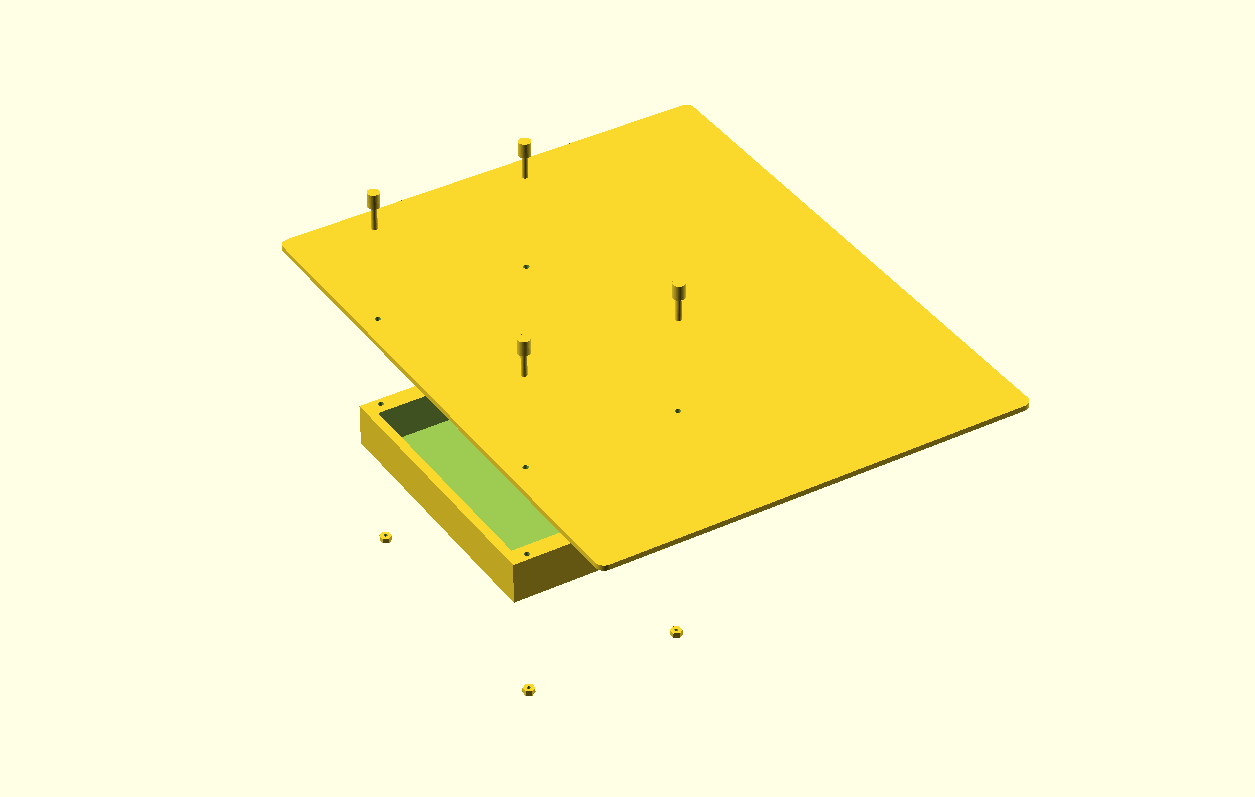
\includegraphics[scale=0.235]{figures/iterations/v5.png}
% \end{minipage}
% % \hspace{0.5cm}
% \begin{minipage}[b]{7.5cm}
% \centering
% 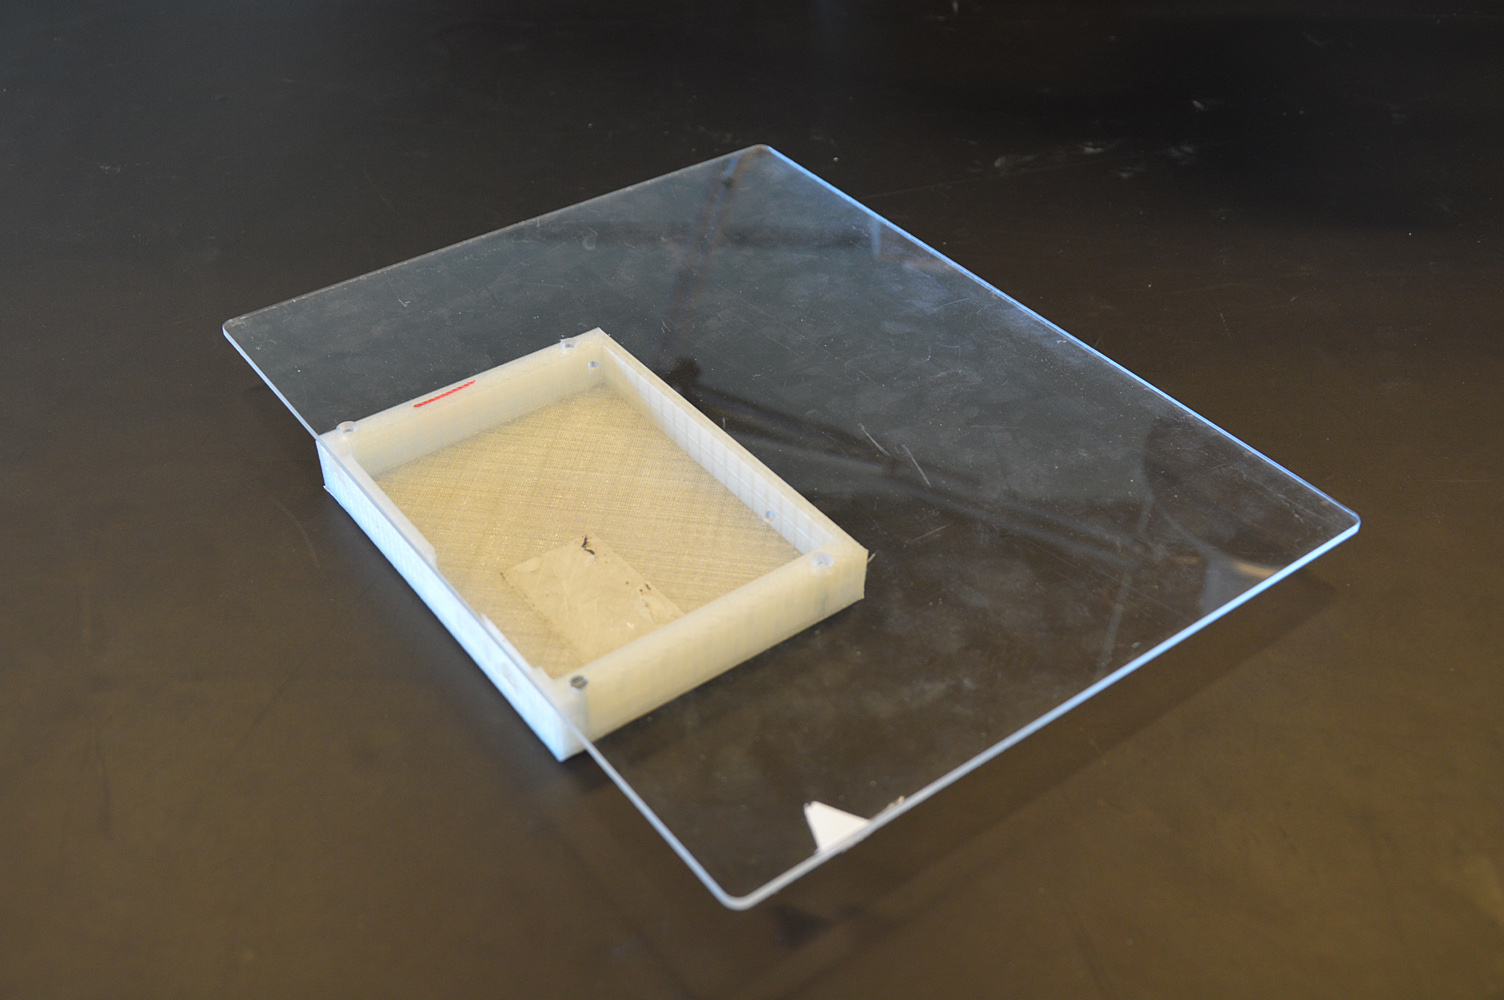
\includegraphics[scale=0.58]{figures/iterations/v5-photo.jpg}
% \end{minipage}
% \caption{\small {\it {The fourth prototype idea}}} \label{fig:v4}
% \end{figure}

% -------------------

\subsubsection{Fourth iteration}

The fourth prototype shown on figure \ref{fig:v5} was the last iteration made within the available time constraint. The electronics compartments were removed, in favour of one single room for the Arduino, Wifi module, RFID reader, and the battery, and another room for the ultrasonic tracker. 

\begin{figure}[h]
\setlength{\belowcaptionskip}{-5mm}
\begin{minipage}[b]{.5\textwidth}
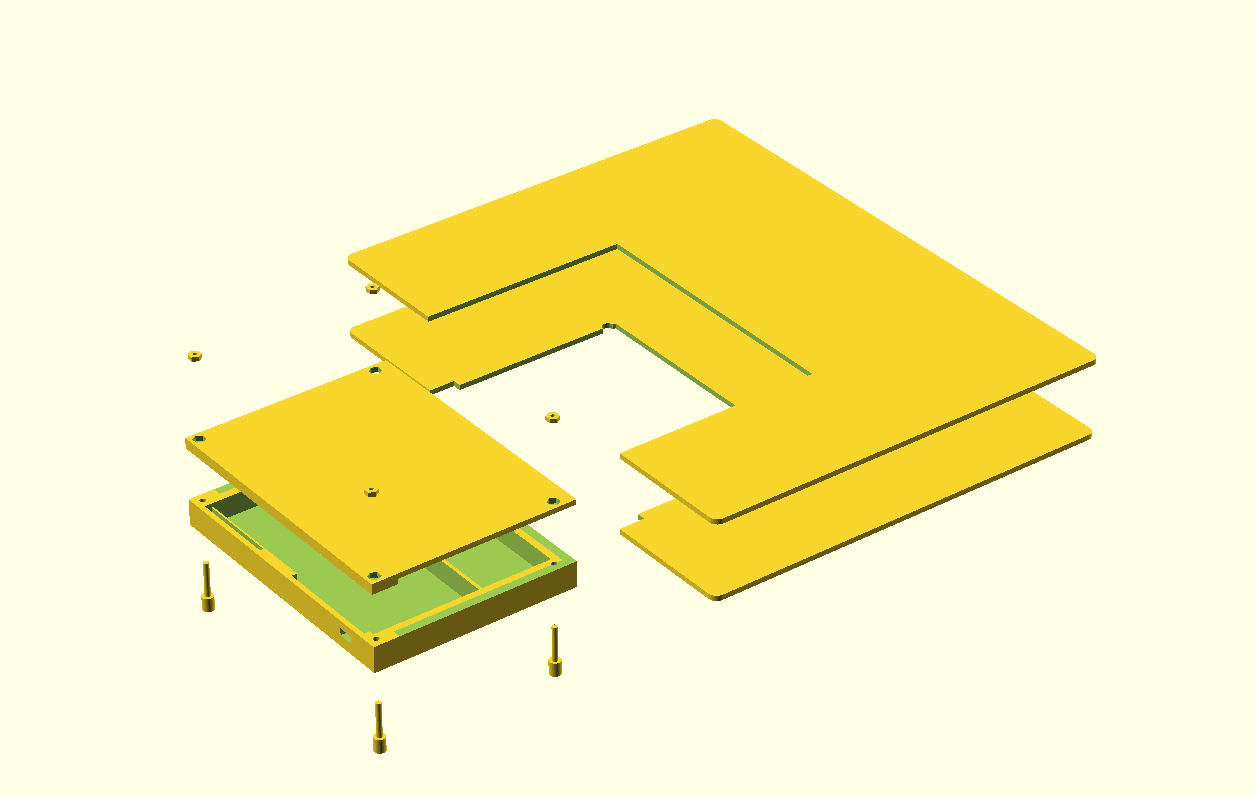
\includegraphics[width=1.05\textwidth]{figures/iterations/v6.png}
\end{minipage}
\begin{minipage}[b]{.5\textwidth}
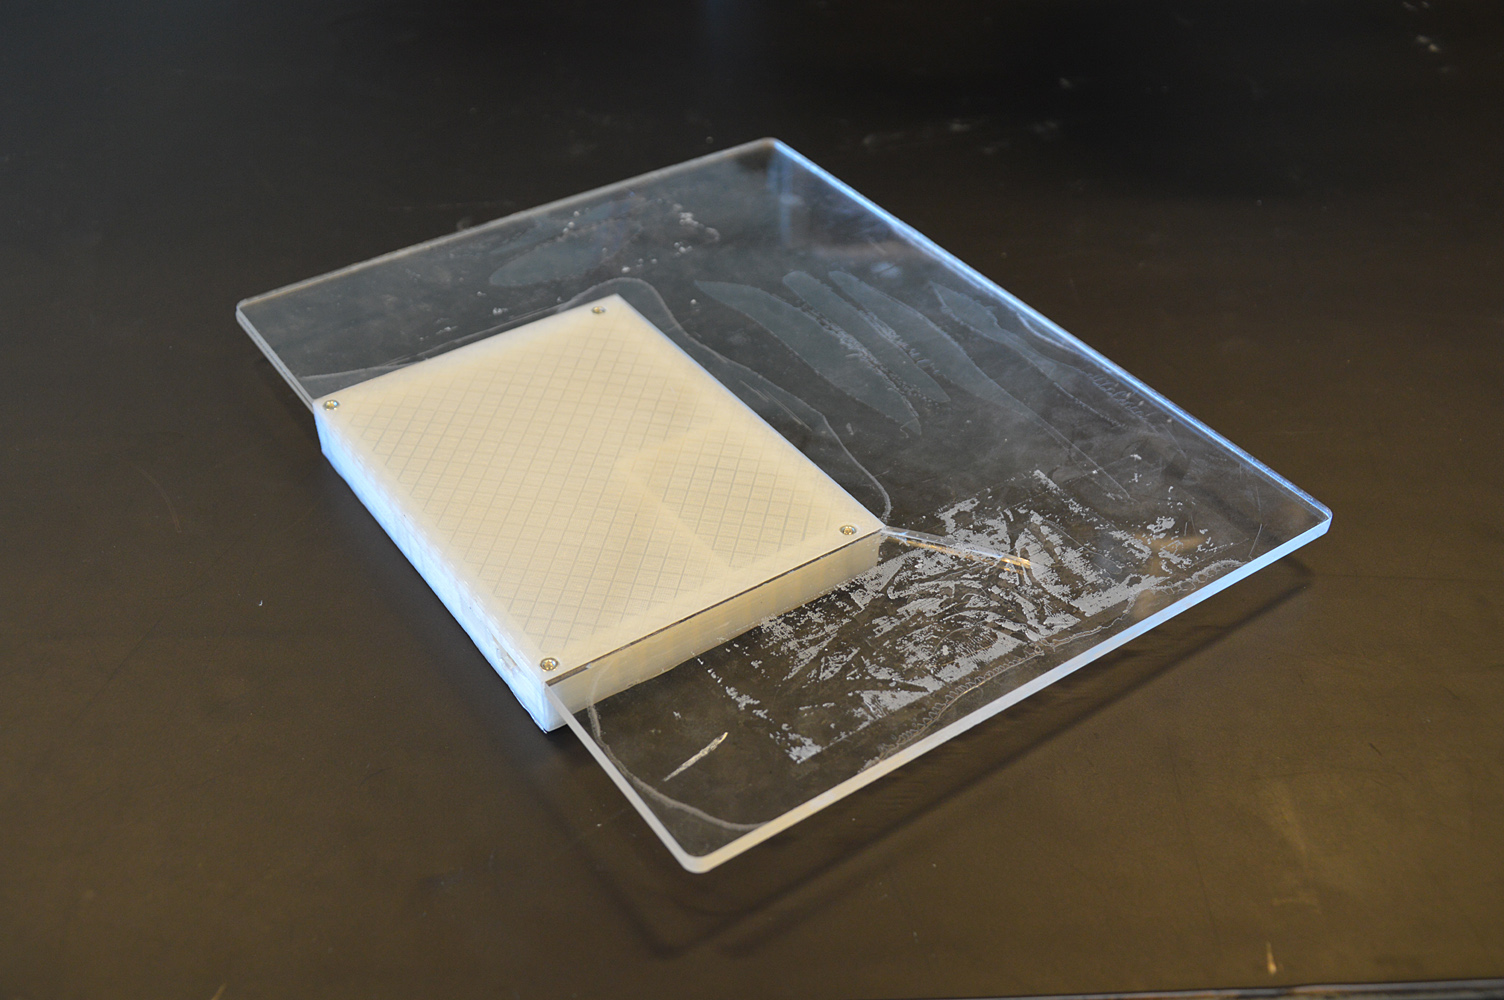
\includegraphics[width=1\textwidth]{figures/iterations/v6-photo.jpg}
\end{minipage}
\caption{\small {\it {The fourth prototype idea}}} 
\label{fig:v5}
\end{figure}

The electronics were now wired on a breadboard, which made the system thinner, and easier to maintain as opposed to single elements wired together. The slide system was also improved, and required no bending acrylic parts - a rail was added to the 3D printed lid, where the acrylic sheet is supposed to slide in. The screws were then tightened, which resulted in tightening the box to the acrylic sheets, thus making it hold on to it. This ensured a way to easily slide the box out, when in need for maintenance. A small hole was added at the bottom, to access the battery charger's battery state button. The PLA chosen for the 3D printing was in this case semi transparent, which allowed to place LEDs behind the material, and see the colours distinctly.

The previous disadvantages were assessed, resulting in the following additional positive observations:

\begin{itemize} \itemsep0em
  \item The electronics were finally able to fit in the box without any hassle.
  \item The slide system worked as intended.
  \item The chosen RGB LED's colours were easily discerned.
\end{itemize}

\begin{figure}[h]
  \setlength{\belowcaptionskip}{-25mm}
  \centering
  \makebox[\textwidth][c]{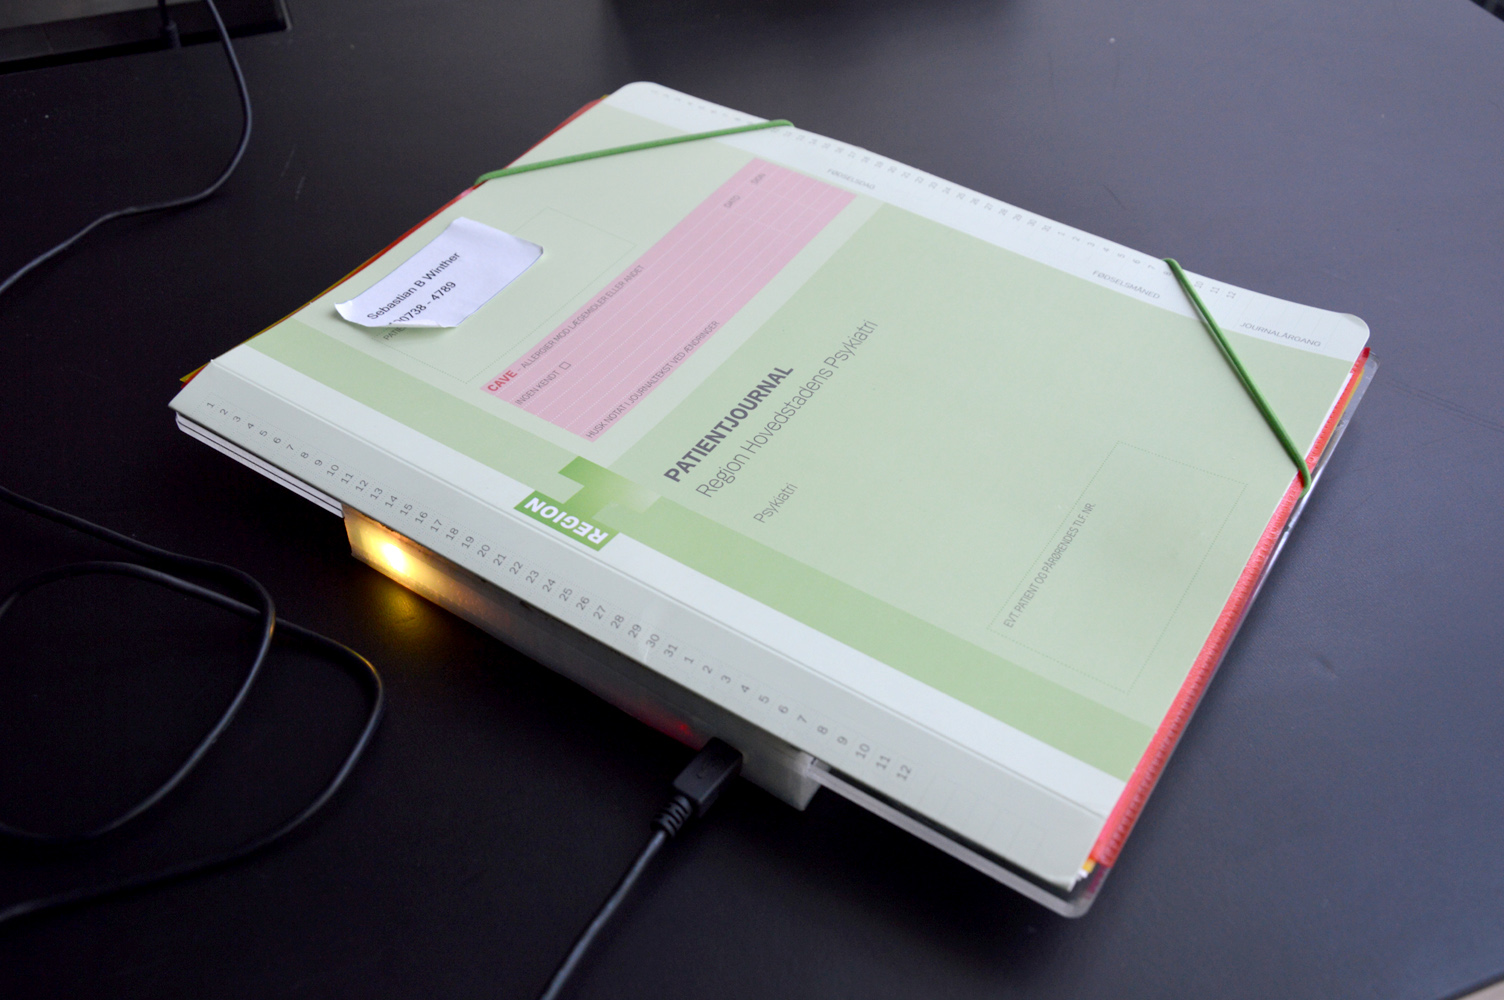
\includegraphics[width=\textwidth]{figures/journal-1.jpg}}
  \caption{\small {\it {The finished Hybrid Patient Record with a paper journal and connected to a charger.}}} 
  \label{fig:journal-1}  
\end{figure}

\clearpage